\section{Konkrete Datenmodelle}
\label{sec:concrete_models}

Neben den Datenmodellen, welche die Informationen beinhalten aus denen der Generator ausführbaren Quellcode erzeugt, wird im folgenden Abschnitt das im Sprachenmodell verwendete Kompositum-Muster erläutert.

\subsection{REST-Modell}
\label{sec:rest_model}

Zuerst muss die abstrakte Beschreibung der Spreadshirt-\gls{API} von der \gls{XML}-Form, bestehend aus einem \gls{WADL} und einem oder mehreren Schemabeschreibungen, in ein für den Generator verarbeitbares Format überführt werden.

Die durch die \gls{WADL}-Datei beschriebene Baumstruktur muss in ein Datenmodell bestehend aus Klassen und Objekten transformiert werden.
Um effektiv mit der \gls{XML} Darstellung arbeiten zu können wird diese zuerst mit einem Parser (\cref{sec:xml_parser}) in ein \emph{Document Object Model} (kurz \textsc{Dom}) überführt, welches im Arbeitsspeicher gehalten wird und damit einen schnellen Zugriff für nachfolgende Operationen darauf erlaubt. In einem nächsten Schritt wird das \textsc{Dom}, welches noch viele \gls{XML} spezifische Informationen enthält, auf die wesentlichen \gls{API} beschreibenden Merkmale reduziert. Im Gegensatz zu der in \cref{fig:wadlstructure} veranschaulichten Webanwendungsbeschreibung werden Referenzen durch deren Definition im Modell ersetzt. Die Klassenamen des Datenmodells orientieren sich an den \gls{WADL} Elementnamen.

\begin{figure}[tb]
    \centering
    \includegraphics[width=0.5\textwidth]{resources/restmodel}
    \caption{\textsc{Uml} Klassendiagramm des \gls{REST}-Modells}
    \label{fig:restmodel}
\end{figure}

Wurzelelement des Modells (\cref{fig:restmodel}) ist die Klasse \classname{Application}, sie enthält \emph{Ressource}-Objekte und den Basisbezeichner der \gls{API} beispielsweise:\\
\texttt{\small http://api.spreadshirt.net/api/v1/}. 

Eine \classname{Ressource}-Klasse enthält eine Menge von \emph{Method}-Objekten sowie einen Ressourcenbezeichner. Dieser ist relativ zum Basisbezeichner des Wurzelelements. Die Ressourcenbezeichner können \emph{Template-Parameter} enthalten. Diese werden bei einer Anfrage durch einen konkreten Wert ersetzt. Beispielweise enthält der Bezeichner für die Ressource eines bestimmten Users den Template-Parameter \texttt{\{userid\}}, vollständiger Ressourcenbezeichner \texttt{users/\{userid\}}. Ressourcenbezeichner werden durch die Klasse \classname{SplitPath} repräsentiert. 

Jede \classname{Method}-Klasse enthält ein \emph{Request} und ein \emph{Response} Objekt. Sie enthalten die nötigen Informationen für den Aufruf der Methode, beziehungsweise über den Aufbau der Antwortnachricht.

Eine \classname{Request}-Klasse enthält eine Liste von Query-Parametern sowie ein \emph{Representation} und \emph{Response} Objekt.

Die Klasse \classname{Parameter} enthält Angaben zum \emph{Style}, Typ, Vorgabewert und ob dessen Angabe \enquote{required}, also notwendig ist. Die Angabe des Typs ist eine Referenz auf einen Typ aus einer \gls{XML}-Schemabeschreibung. Der \emph{Style} gibt an wie der Parameter übermittelt wird, als Teil der Query \texttt{?mediaType=xml}, \emph{Key-Value Pair} des \gls{HTTP}-Header oder als \emph{Template-Parameter} des Ressourcenbezeichners. 

Die Klasse \classname{Response} enthält eine Liste mit \emph{Representation} und Parameter Objekten. Die Objekte vom Typ Representation enthalten die Beschreibung der Daten, die bei einer erfolgreichen Anfrage an die Ressource zurückgesendet werden sowie die der Fehlermeldung, welche der Client anderenfalls erhält. Zwischen einer Fehlermeldung und einer erfolgreichen Anfrage kann anhand des Werts des \gls{HTTP}-Statuscodes unterschieden werden. Erfolgreiche Anfragen liefern in der Antwort meist einen Statuscode 200 \classname{OK} oder 201 \classname{Created} zurück, abhängig von der Anfragemethode. Die Response Parameter geben Einträge im \gls{HTTP}-Header an, welche für den Client nützliche Informationen enthalten. Legt der Client z.B. via \textsc{Post} auf der Ressource \texttt{sessions} eine neue \gls{API}-Session an, so enthält das Feld \texttt{Location} des \gls{HTTP}-Headers der Serverantwort eine \gls{URL} auf die Ressource der angelegten Session.

Die \classname{Representation}-Klasse dient zur Beschreibung der Daten, welche entweder zur \gls{API} gesendet oder von dieser empfangen werden, sie besteht aus einer Angabe des \emph{media-type}, des \gls{HTTP}-Statuscodes und eine Referenz auf die Definition des Datentyps. Das \emph{Representation}-Objekt des Request einer \textsc{Put}- oder \textsc{Post}-Methode charakterisiert zum Beispiel den Aufbau der Daten, welche der Ressource übermittelt werden, üblicherweise im \gls{HTTP}-Body. Die Charakterisierung erfolgt dabei in Form einer Referenz auf einen Typ aus einer Schemabeschreibung sowie der Angabe des \emph{media-type}. Beispielsweise enthält das \emph{Representation}-Objekt der \textsc{Put}-Methode auf Ressource \texttt{users/\{userId\}/designs/\{designId\}} den media-type \texttt{application/xml} und eine Referenz auf den Typ \texttt{sns:design}. 

Referenzen auf Typdeklaration aus einer Schemabeschreibung werden nachfolgend im Modell durch die konkrete Deklaration des Typs aus der \gls{XML}-Schemabeschreibung ersetzt, \cref{sec:application_model}. 

Ein Objekt der \classname{Doc}-Klasse enthält einen Titel und eine Kurzbeschreibung des zugehörigen Elements.
Der Generator erzeugt daraus Quellcodekommentare für die Dokumentation der Bibliothek.

\subsection{Schema-Modell}
\label{sec:schema_model}

\begin{figure}[t]
    \centering
    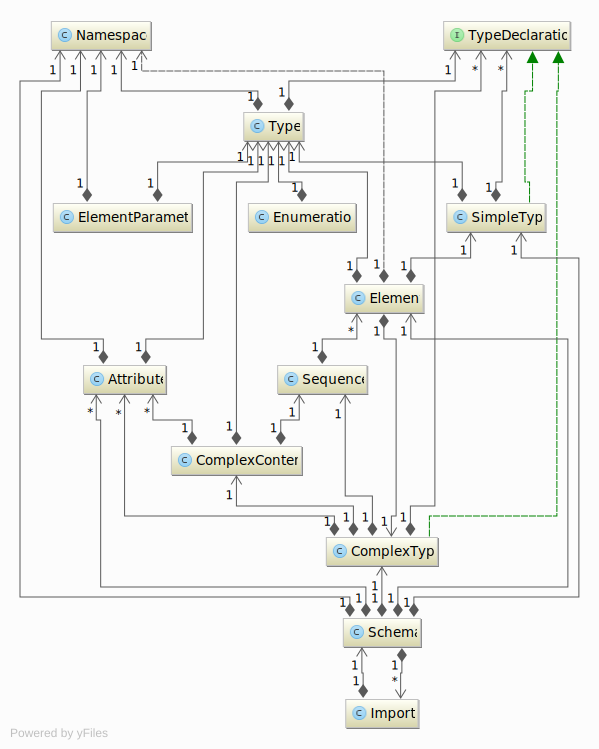
\includegraphics[width=0.6\textwidth]{resources/typemodel}
    \caption{\textsc{Uml} Klassendiagramm des Schemadatenmodells}
    \label{fig:schema_model}
\end{figure}

Wurzel des Schemadatenmodells ist die Klasse \textbf{Schema}. Ein Schema kann Objekte vom Typ \emph{Complex-} und \emph{SimpleType} sowie \emph{Attribute} und \emph{Element} enthalten.

\textsc{Xsd}-Dateien (siehe \cref{sec:xsd}) erlauben das importieren anderer Schemadefinitionen, die Klasse \textbf{Import} ermöglicht dies im Schemamodell. Sie besitzt ein Objekt des zu importierenden Schemas sowie eine \gls{URI} auf die zugehörige \textsc{Xsd}-Datei.

Primitive Schematypen werden durch die Klasse \emph{SimpleType} abgebildet. Objekte dieser Klasse enthalten eine Kennzeichnung der Art des SimpleType (Enumerator, Liste, einfacher Wert) und bei Enumeratoren zusätzlich die einzelnen Enumeratorwerte, sowie die Angabe des Basisdatentyps.

Die \textbf{ComplexType}-Klasse repräsentiert die gleichnamigen strukturierten Typen aus der Schemabeschreibung. 
Ein ComplexType kann Attribute, Elemente, Elementsequenzen und strukturierten Inhalt (\emph{ComplexContent}) enthalten.

\textbf{ComplexContent} kann die gleichen Objekte wie \emph{ComplexType} enthalten, sowie einen Basistyp der Erweitert oder Eingeschränkt wird (\enquote{derivation by extension/restriction}).

Attribute werden durch die gleichnamige Klasse \textbf{Attribute} gekapselt, sie besitzen einen Attributnamen sowie eine Definition ihres Typs.

Elementsequenzen werden durch die \textbf{Sequence}-Klasse repräsentiert. Sie enthält einen Reihenfolgeindikator (siehe \cref{sec:xsd}) und die Elemente der Sequenz.

Objekte der Klasse \textbf{Element} besitzen einen Bezeichner, sowie einen Complex- oder SimpleType und optional eine Angabe der Auftrittshäufigkeit. Die Klasse \emph{ElementParameter} dient nur zur Kapselung der Daten welche an den Konstruktor der Elementklasse gegeben werden.

Durch die Klasse \textbf{Namespace} werden der Namensraumbezeichner und der konkrete Namensraum eines Typs aus dem Schema gekapselt. 

\begin{figure}[ht]
    \centering
    \begin{minipage}[b]{0.50\linewidth}
        \begin{lstlisting}[
            language=XML,
            caption=Point Datentyp aus der Spreadshirt-\textsc{Api} Schemabeschreibung,
            label=lst:xsdExamplePoint,    
            basicstyle=\tiny\ttfamily,
            numbers=none,
            xleftmargin=0mm,
            framexleftmargin=2mm,
        ]
<xs:element 
    xmlns:tns="http://api.spreadshirt.net" 
    type="tns:point" name="point"/>

<xs:complexType name="point">
    <xs:sequence>
        <xs:element type="xs:double" name="x"/>
        <xs:element type="xs:double" name="y"/>
    </xs:sequence>
    <xs:attribute 
        xmlns:tns="http://api.spreadshirt.net" 
        type="tns:unit" name="unit"/>
</xs:complexType>
        \end{lstlisting}
    \end{minipage}
    \quad    
    \begin{minipage}[b]{0.45\linewidth}
        \begin{tikzpicture}[every tree node/.style={font=\tiny}]
            \Tree
            [
                .Element
                [
                    .ComplexType
                    [ . Attribute ]
                    [ .Sequence 
                        Element
                        [ .Element ]
                    ]
                ]
            ]
        \end{tikzpicture}
        \caption{Klassendarstellung des Datentyps Point im Schemamodell}
        %\label{fig:minipage2}
    \end{minipage}
\end{figure}

\subsection{Applikationsmodell}
\label{sec:application_model}

Das Applikationsmodell ist die Gesamtheit des \textsc{Rest}- und Schemamodells. Referenzen auf Typenbeschreibungen im \textsc{Rest}-Modell werden durch deren Definition im Schemamodell ersetzt. Dieses gemeinsame Modell dient dem Generator als Eingabequelle.

\subsection{Sprachenmodell}
\label{sec:language_model}

\begin{sidewaysfigure}
    \centering
    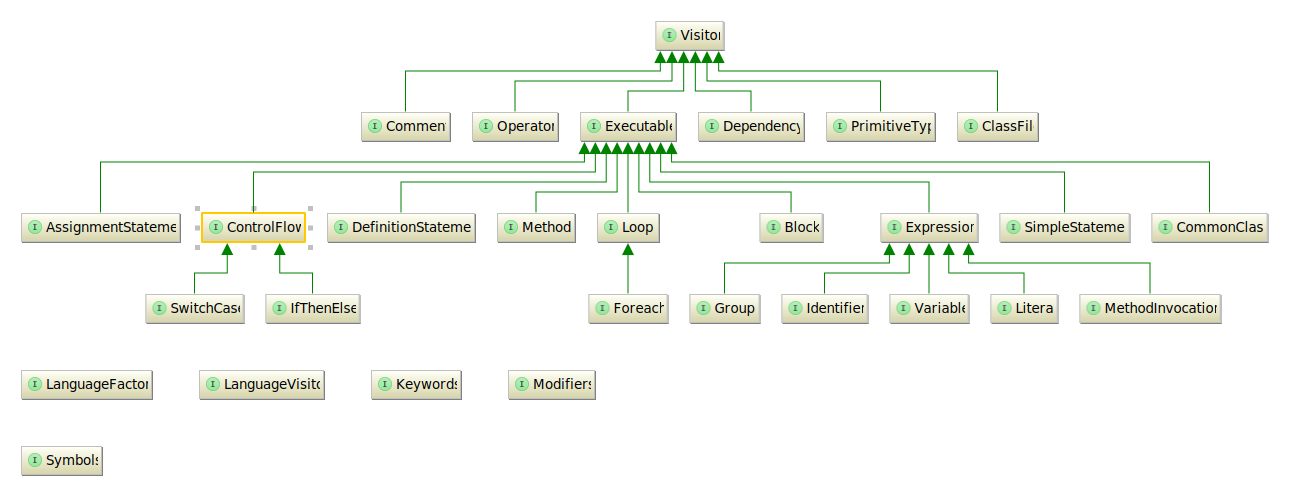
\includegraphics[width=\textheight]{resources/languagemodel_common}
    \caption{\textsc{Uml} Klassendiagramm des Zielsprachenmodells}
    \label{fig:language_model}
\end{sidewaysfigure}

Um die gewünschte Austauschbarkeit der Zielsprache zu gewährleisten wurde ein abstraktes Sprachenmodell entworfen welches die Konstrukte einer dateibasierten objektorientierten Programmiersprache abbildet. 
%Anforderungen erstellen und referenzieren.
Die gewünschte Zielsprache muss dabei die Klassen und Methoden des Modells implementieren sowie eine \emph{Language Factory} (\cref{sec:language_factory}) bereitstellen um vom Generator genutzt werden zu können.
Um Semantik und Syntax der Zielsprache im Modell zu trennen --- abgesehen von Symbolen und Schlüsselwörtern --- wird die Syntax in der Klasse \emph{LanguageVisitor} (\cref{sec:language_visitor}) gekapselt. Das Sprachenmodell kapselt somit die Semantik der Zielsprache.

Alle Interfaces des Modells (\cref{fig:language_model}) erweitern das Interface \classname{Visitor}. Somit ist sichergestellt, dass alle Klassen, die diese Schnittstellen implementieren, eine \emph{accept}-Methode für den \emph{LanguageVisitor} bereitstellen.

Basis des Modells ist das Interface \classname{ClassFile}. Es abstrahiert eine Klassendatei mit den Eigenschaften:
\begin{compactitem}
    \item Dateiname
    \item Namensraum
    \item Liste von Abhängigkeiten (\emph{Dependency}-Klasse)
    \item Klassendefinition
\end{compactitem}

Die Liste von Abhängigkeiten der zu generierenden Klassen muss vorher aus dem Eingabemodell ermittelt werden. Dies geschieht durch Analyse der in den Elementdefinitionen des Schemamodells enthaltenen Typen. 

\classname{Dependency} enthält das Schlüsselwort oder Methodenaufruf zum Import einer Quellcodedatei. In \textsc{Php} werden solche Dateien bpsw. so importiert: \texttt{require\_once("foo.php");}.

\classname{Executable} implementieren alle Elemente der Zielsprache die \enquote{ausführbar} sind. Das Modell unterscheidet dabei zwischen \emph{Ausdruck} und \emph{Anweisung}. 

Das Interface \classname{CommonClass} dient der Implementierung einer Klassendefinition. Da das Interface selbst \emph{Statement} erweitert, kann eine Klasse weitere Klassendefinitionen beinhalten. Eine Klassendefinition besteht dabei aus einem Klassename, Modifiers und aus einer Menge von Statements:
\begin{compactitem}
    \item \emph{DefinitionStatement} zur Einführung von lokalen Variablen.
    \item \emph{Method} zur Definition von Methoden.
\end{compactitem}

Das \classname{Modifier}-Interface deklariert Methoden um die Schlüsselwörter für \emph{Sichtbarkeitsmodifikatoren} (\enquote{Access Modifier}) und \enquote{Non Access Modifiers} wie \texttt{static} oder \texttt{final} zu erhalten.

Durch das \classname{Method}-Interface kann eine Methodendefinition implementiert werden. Eine Methode beinhaltet dabei:
\begin{compactitem}
    \item Modifier
    \item Methodenname
    \item Rückgabetyp
    \item Liste von Parametern (Parameter können dabei alle Klassen sein die \emph{Expression} implementieren)
    \item \emph{Block}
\end{compactitem}

Ein \classname{Block} kapselt eine Menge von Statements.

Operatoren der Zielsprache müssen das Interface \classname{Operator} implementieren, ein Operator ist durch seine Arität (Stelligkeit), Notation und sein Symbol gekennzeichnet. Zum Beispiel ist der Dereferenzierungsoperator in \textsc{Php} \emph{zweistellig}, \emph{Infix} notiert und durch das Symbol \texttt{->} gekennzeichnet.

Die Interfaces \classname{Keywords} und \classname{Symbols} dienen zur Kapselung der Schlüsselwörter und Symbole einer Sprache. Keywords enthält Methoden zur Abfrage typischer Schlüsselworte wie \texttt{class}, \texttt{import}, \texttt{new} oder \texttt{this}. Sprachspezifische Symbole wie \emph{Verkettungs}- und \emph{Scope}-Operatoren oder Präfixe für Variablennamen können über Methoden der Klasse Symbols vom Generator abgefragt werden.

\subsubsection{Kompositum-Pattern im Sprachenmodell}
\label{sec:composite_pattern}

Zweck des Composite- oder auch Kompositum-Patterns ist die Gleichbehandlung von Einzelelementen und Elementgruppierungen in einer verschachtelten Struktur
(z. B. Baum), sodass aus Sicht des Clients keine explizite Unterscheidung
notwendig ist (nach \cite[][S. 102]{patternsKompakt}).

Anwendung fand das Pattern an zwei Stellen im Modell, erstens in den Klassen welche \classname{Expression} und zweitens, welche \classname{Statement} implementieren.
Ein Beispiel für den Aufbau eines Ausdrucks durch Klassen des Interface \emph{Expression} aus dem Sprachenmodell zeigt \cref{fig:example_expression}. Von \emph{Statement} abgeleitete Klassen können ebenso eine Baumstruktur bilden. \emph{Block} kann beispielsweise selbst wieder Codeblöcke --- also Statements vom Typ Block --- enthalten. 

\begin{figure}
    \[
        \overbrace{
            \underbrace{
                \overset{\text{Identifier}}{x} \underset{\text{Operator}}{+} \overset{\text{Identifier}}{y}
            }_{\text{SimpleExpression}} 
            \underset{\text{Operator}}{/}
            \underbrace{
                ( 
                    \underbrace{
                        \overset{\text{Literal}}{1.2} \underset{\text{Operator}}{*} \overset{\text{Literal}}{4}
                    }_{\text{SimpleExpression}} 
                )
            }_{\text{Group}}
        }^{\text{SimpleExpression}} 
    \]   
    \caption{Beispiel für den Aufbau einer \enquote{Expression} im Sprachenmodell}
    \label{fig:example_expression}
\end{figure}
